\documentclass[tikz,border=10pt]{standalone}
\usepackage{tikz}
\begin{document}
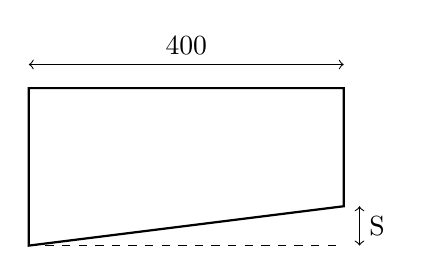
\begin{tikzpicture}
    % Draw the trapezoid with the inclined bottom side slanting upwards from left to right
    \draw[thick] (0,0) -- (4,0.5) -- (4,2) -- (0,2) -- cycle;

    % Draw the horizontal dimension line with "400" at the top
    \draw[<->] (0,2.3) -- (4,2.3) node[midway, above] {400};

    % Draw the horizontal dotted line at the bottom, parallel to the top side
    \draw[dashed] (0,0) -- (4,0);
    
    % Draw the vertical dimension line for "S" on the right side
    \draw[<->] (4.2,0) -- (4.2,0.5) node[midway, right] {S};
\end{tikzpicture}
\end{document}
